%%%%%%%%%%%%%%%%%%%%%%%%%%%%%%%%%%%%%%%%%
% University/School Laboratory Report
% LaTeX Template
% Version 3.0 (4/2/13)
%
% This template has been downloaded from:
% http://www.LaTeXTemplates.com
%
% Original author:
% Linux and Unix Users Group at Virginia Tech Wiki
% (https://vtluug.org/wiki/Example_LaTeX_chem_lab_report)
%
% License:
% CC BY-NC-SA 3.0 (http://creativecommons.org/licenses/by-nc-sa/3.0/)
%
%%%%%%%%%%%%%%%%%%%%%%%%%%%%%%%%%%%%%%%%%

%----------------------------------------------------------------------------------------
%	PACKAGES AND DOCUMENT CONFIGURATIONS
%----------------------------------------------------------------------------------------

\documentclass{article}

\usepackage{mhchem} % Package for chemical equation typesetting
\usepackage{siunitx} % Provides the \SI{}{} command for typesetting SI units
\usepackage{hyperref}
\usepackage{graphicx} % Required for the inclusion of images
\usepackage{tabularx}
\usepackage{float}
\usepackage{algorithm}
\usepackage{algpseudocode}
\usepackage{bm}
\usepackage{multirow}% http://ctan.org/pkg/multirow
\usepackage{hhline}% http://ctan.org/pkg/hhline
\usepackage{caption}
\usepackage{subcaption}
\usepackage{listings}
\usepackage{xcolor}
\lstset{
    numbers=left,
    stepnumber=1,    
    firstnumber=1,
    numberfirstline=true,
    basicstyle=\ttfamily,
    keywordstyle=\color{blue}\ttfamily,
    stringstyle=\color{red}\ttfamily,
    commentstyle=\color{green}\ttfamily,
    breaklines=true,
}


\setlength\parindent{0pt} % Removes all indentation from paragraphs

\renewcommand{\labelenumi}{\alph{enumi}.} % Make numbering in the enumerate
% environment by letter rather than number (e.g. section 6)

%\usepackage{times} % Uncomment to use the Times New Roman font

%----------------------------------------------------------------------------------------
%	DOCUMENT INFORMATION
%----------------------------------------------------------------------------------------

\title{UC Davis STA 242 2015 Spring Assignment 4~\cite{wu2015bmlgrid_v1.1}} %
% Title
\author{Wenhao \textsc{Wu}, 998587583} % Author name
\date{\today} % Date for the report

\begin{document}
\maketitle % Insert the title, author and date

% If you wish to include an abstract, uncomment the lines below

\section{Implementation of \texttt{crunBMLGrid()}}
In order to highlight the performance difference between R and C++
implementation of BML simulation, we implement 2 versions of the BML simulator
routine:
\begin{itemize}
    \item \texttt{crunBMLGrid1()}: rewrite the entire \texttt{runBMLGrid()} in
    C++.
    \item \texttt{crunBMLGrid2()}: rewrite only the 2 key routines to get the
    next location of cars (\texttt{idx\_right()} and \texttt{idx\_up()}) with
    C++.
\end{itemize}
The overall algorithm design for both functions are very similar to the original
R function \texttt{runBMLGrid()}. However, the R's vectorized operations are
rewritten with C++ for-loops. As suggested by the example ``R vectorisation vs.
C++ vectorisation'' in~\cite{wickham2014advanced}, one advantage of C++ for-loop
implementation over the R vecotrized operation is that it might need to create less
intermediate vector variables. Since our original 2 routines,
\texttt{idx\_right()} and \texttt{idx\_up()}, both contains a few vectorized
mathematic operations, we expect to achieve some performance gain with
\texttt{crunBMLGrid2()}. Another main advantage of C++ over R is that it allows
more efficient memory management~\cite{xian2014efficient}: in our original
\texttt{runBMLGrid()} when ever the grid \texttt{g} or the cars' locations \texttt{red} and \texttt{blue}
is updated, R creates a new object instead of modifying in-place (as verified
with function \texttt{address()} from package 'pryr'). This might
results in a lot of redundant memory management operations under the hood. In
\texttt{crunBMLGrid1()}, we use in-place modification whenever possible, which
is mainly achieved by using reference inputs for self-defined functions. To
interface our C++ functions and R we make use of package `Rcpp'.

\section{Verification}
We first verify qualitatively the behavior of BML model computed with our new
C++ routines. As in our previous assignment, We pick a
$r=100$, $c=99$ grid in which the number of blue cars and red cars are the same. After $N =
10000$ steps, the final states of the grid for $\rho = 0.2, 0.33, 0.38, 0.43,
0.5$ returnd by \texttt{crunBMLGrid1()} are plotted in
Fig.~\ref{fig:final_state}, where we observe the same chaotic phenomenon as the
results computed with our original \texttt{runBMLGrid()} routine.
\texttt{crunBMLGrid2()} returns a similar results and is thus omitted.

We further verify that \texttt{crunBMLGrid1()}, \texttt{crunBMLGrid2()} and
\texttt{runBMLGrid()} return identical results given the same inputs with
package 'testthat'. Besides the degenerated cases, in a $r=100$, $c=99$
grid we test 6 different cases where there are different numbers of red and blue
cars. For each case, we randomly generate 5 instances of initial grid
\texttt{g}. Our tests make sure that both \texttt{crunBMLGrid1()} and
\texttt{crunBMLGrid2()} return identical results after $N = 10000$ steps for all
30 instances. We have also manually checked that, upon early break from the
outer for-loop due to grid lock when $\rho$ is large, the number of steps executed
before breaking are the same for all 3 routines.

\section{Running Time Comparison with R's Vectorized Operation}
To compare the performance of \texttt{crunBMLGrid1()} and
\texttt{crunBMLGrid2()} with \texttt{runBMLGrid()}, we measure the running time
of all the three functions for $r=c=128,256,512,1024$ and
$\rho=0.1,0.2,9.3,0.4,0.5,0.6,0.7$. For each of the $4\times7=28$ settings we
randomly generate 20 initial grids and apply \texttt{crunBMLGrid1()},
\texttt{crunBMLGrid2()} and \texttt{runBMLGrid()} on them and record the running
time. We also fix the number of steps to $N=10000$ and have the same number of
red and blue cars in the grid. Again we run this test on a Dell Precision T1700
workstation equipped with 16GB DDR3 RAM and a Core i7-4790K CPU in Ubuntu 14.04
OS. The average and error bar of the running time in seconds and the relative
speed up of the average running time from \texttt{runBMLGrid()} to
\texttt{crunBMLGrid1()} and \texttt{crunBMLGrid2()} are plotted in
Fig.~\ref{fig:running_time} and Fig.~\ref{fig:speed_up}, repectively.
We have also plotted the running time for different number of steps of $N$ for
$\rho=0.3, 0.4, 0.5$ and $r=c=256$ in Fig.~\ref{fig:running_time_vs_numsteps}.
The main results are summarized as follows:
\begin{itemize}
    \item For \texttt{crunBMLGrid2()} where only the key routines are rewritten
    in C++, there is a limited speed up of less than 2x, and this speed up
    remains relatively constant for different $\rho$, $l$ and $N$.
    \item For \texttt{crunBMLGrid1()} which is entirely rewritten in C++, there
    is a significant speed up from 3x to 9x. In general, the larger the edge
    length, the smaller the speed up is. The speed up for cases where there is
    no grid lock detected is significantly higher than the cases where there is
    grid lock and early breaks. Surprisingly, the peak of running time for both
    \texttt{runBMLGrid()} and \texttt{crunBMLGrid2()} appears at $\rho = 0.3$,
    yet that for \texttt{crunBMLGrid1()} appears at $\rho = 0.4$ (In our
    running time test we have also verified that all 3 functions returned the
    same results). In Fig.~\ref{fig:running_time_vs_numsteps} we further
    verified that when $\rho = 0.4$, $N=1000$, even though for all the 20
    initial grids the early break has not been detected, the relative speed up
    ($\sim4$x) has already been much lower than that when $\rho = 0.3$. This
    indicates that the sharp drop of speed up in Fig.~\ref{fig:speed_up} has
    nothing to do with the grid-detection mechanism in our algorithm. Our best
    guess is that it has something to do with R's or Rcpp's memory management
    schemes.
    \item From Fig.~\ref{fig:running_time}
    and Fig.~\ref{fig:running_time_vs_numsteps}, we notice that when the BML
    model is in ordered state ($\rho < 0.4$), the variances of the running time
    of all 3 routines are very small among different initial states. When the
    BML model is in the critical state ($\rho \approx 0.4$), the variances of
    the running time are very large since different initial states of the grid
    may lead to significantly different early break time (if there is grid lock
    detected). When the BML model is in the stale state ($\rho > 0.4$), as
    $\rho$ grows, the variances of running time begin to decrease since most
    initaial grid states causes the grid to enter the grid lock mode after only
    a few steps.
\end{itemize}


\section{Conclusion}
Based on the above results, our conclusion is
\begin{itemize}
    \item In this assignment, it is not worth rewriting the key routines in C++
    as in \texttt{crunBMLGrid2()}, since the performance improvement is very
    limited.
    \item Although \texttt{crunBMLGrid2()} offers considerable speed up, in my
    opinion it is still not worth rewriting the entire routine in C++. First of
    all, unless we are dealing with really time-consuming simulation, R's
    advantage of agile development will outweigh the greater running speed of
    C++ routine. Also it is more difficult for C++ routine to return
    differen types of outputs given different inputs. Finally, it is more
    difficult to add other functionalities (such as animation) to the C++
    routines not being able to use the abundant R packages.
    \item It is not worth implementing the grid creation function in C since
    this is not a compuation-intensive routine.
\end{itemize}

%   BIBLIOGRAPHY
%----------------------------------------------------------------------------------------

\bibliographystyle{unsrt}
\bibliography{myrefs}

\begin{figure}[H]
    \begin{minipage}[b]{0.5\linewidth}
      \centering
      \centerline{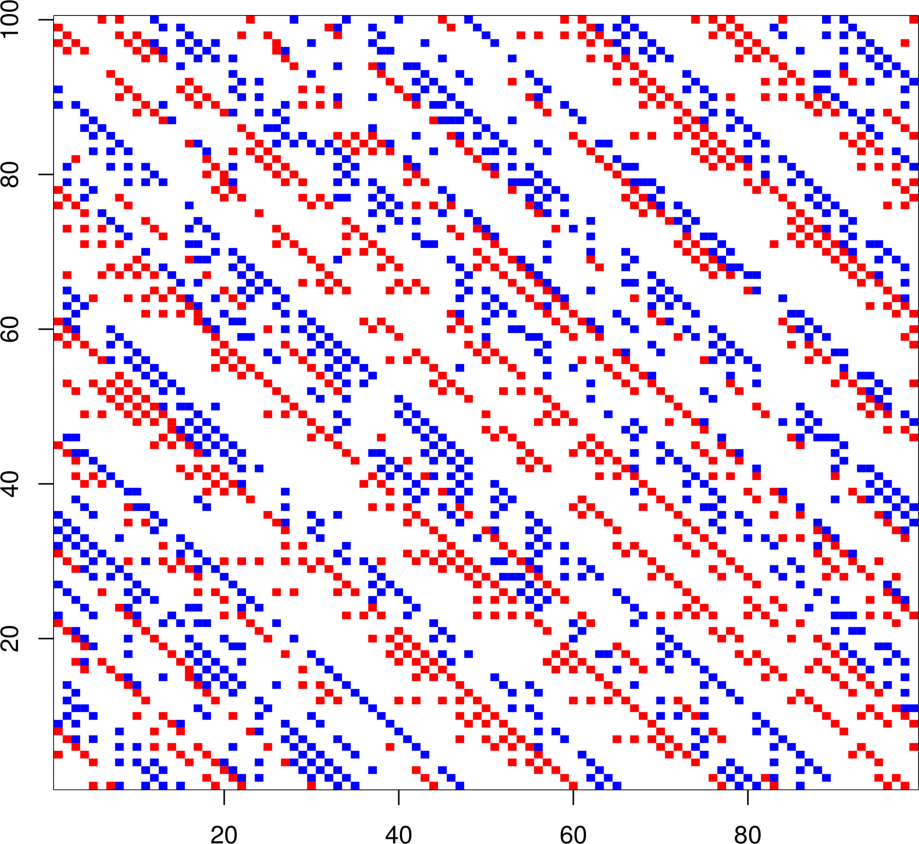
\includegraphics[width=6.0cm]{./figs/TestBehavior_100_99_10000_02_end.pdf}}
      \centerline{(a) $\rho = 0.2$}\medskip
    \end{minipage}
    \hfill
    \begin{minipage}[b]{0.5\linewidth}
      \centering
      \centerline{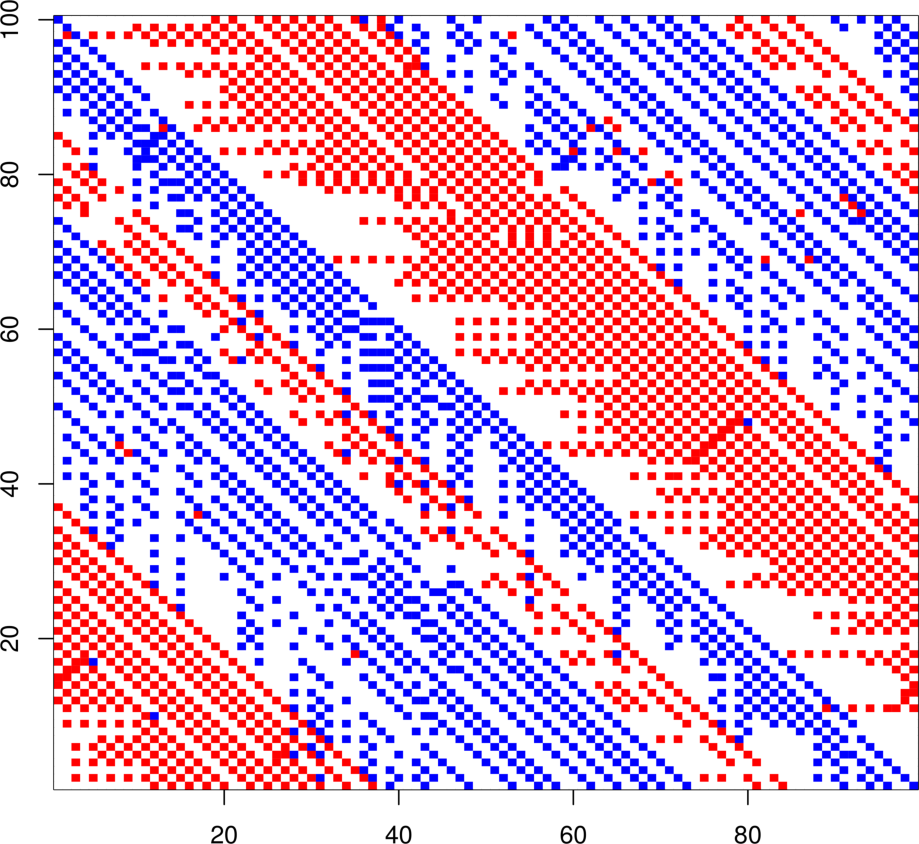
\includegraphics[width=6.0cm]{./figs/TestBehavior_100_99_10000_033_end.pdf}}
      \centerline{(b) $\rho = 0.33$}\medskip
    \end{minipage}
    \hfill
    \begin{minipage}[b]{0.5\linewidth}
      \centering
      \centerline{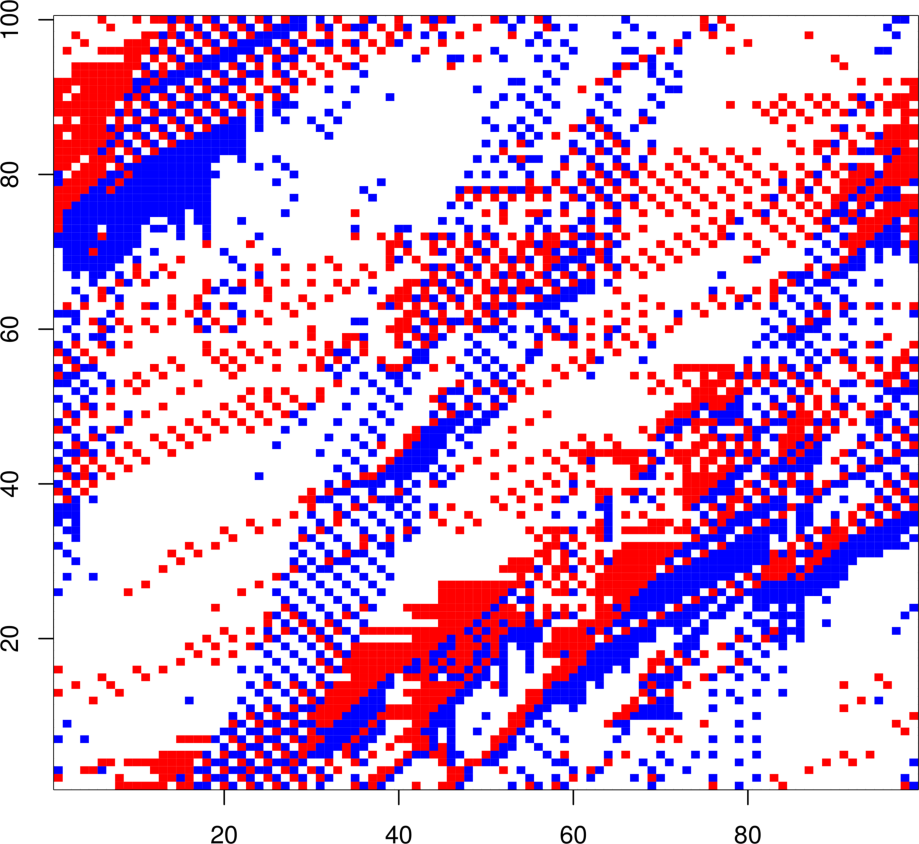
\includegraphics[width=6.0cm]{./figs/TestBehavior_100_99_10000_038_end.pdf}}
      \centerline{(c) $\rho = 0.38$}\medskip
    \end{minipage}
    \hfill
    \begin{minipage}[b]{0.5\linewidth}
      \centering
      \centerline{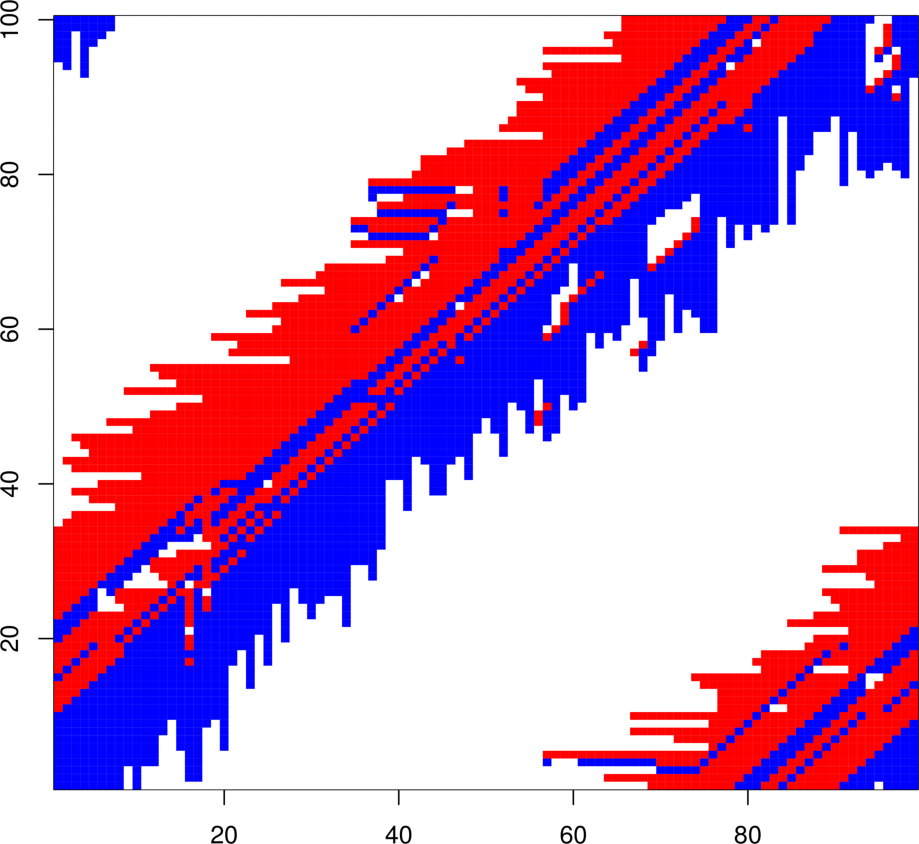
\includegraphics[width=6.0cm]{./figs/TestBehavior_100_99_10000_043_end.pdf}}
      \centerline{(d) $\rho = 0.43$}\medskip
    \end{minipage}
    \hfill
    \begin{minipage}[b]{1\linewidth}
      \centering
      \centerline{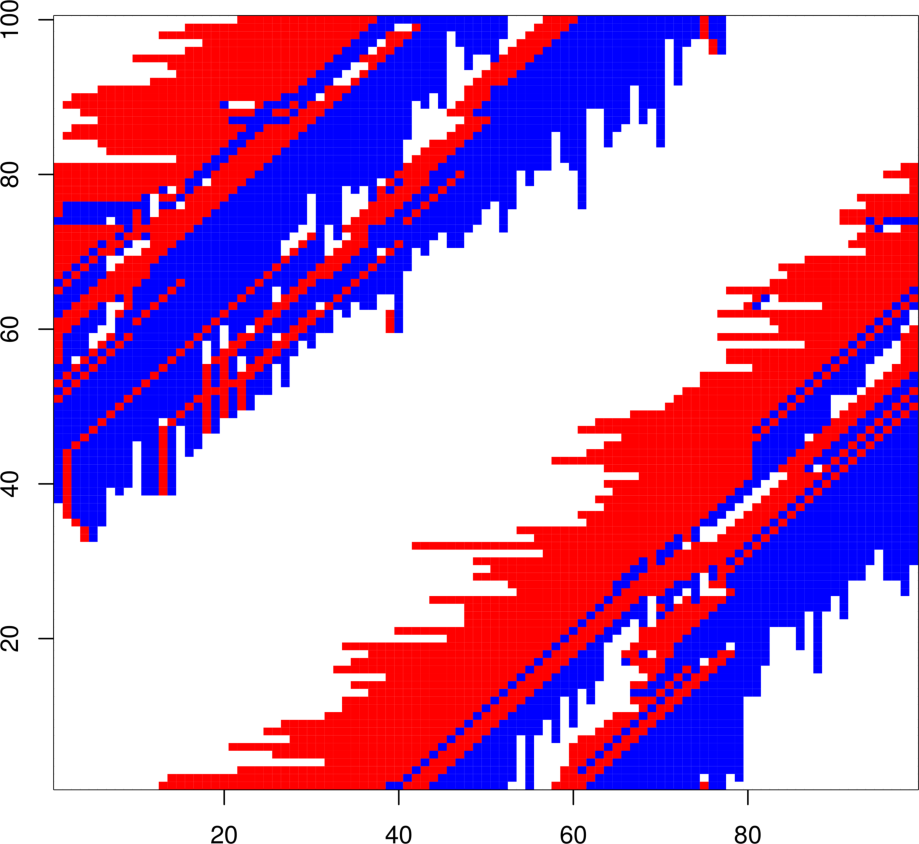
\includegraphics[width=6.0cm]{./figs/TestBehavior_100_99_10000_05_end.pdf}}
      \centerline{(e) $\rho = 0.5$}\medskip
    \end{minipage}
    \caption{Final state of a $100\times99$ grid with equal number of blue and
    red cars after 10000 steps for different car density $\rho$.}
    \label{fig:final_state}
\end{figure}

\begin{figure}[H]
    \begin{minipage}[b]{0.5\linewidth}
      \centering
      \centerline{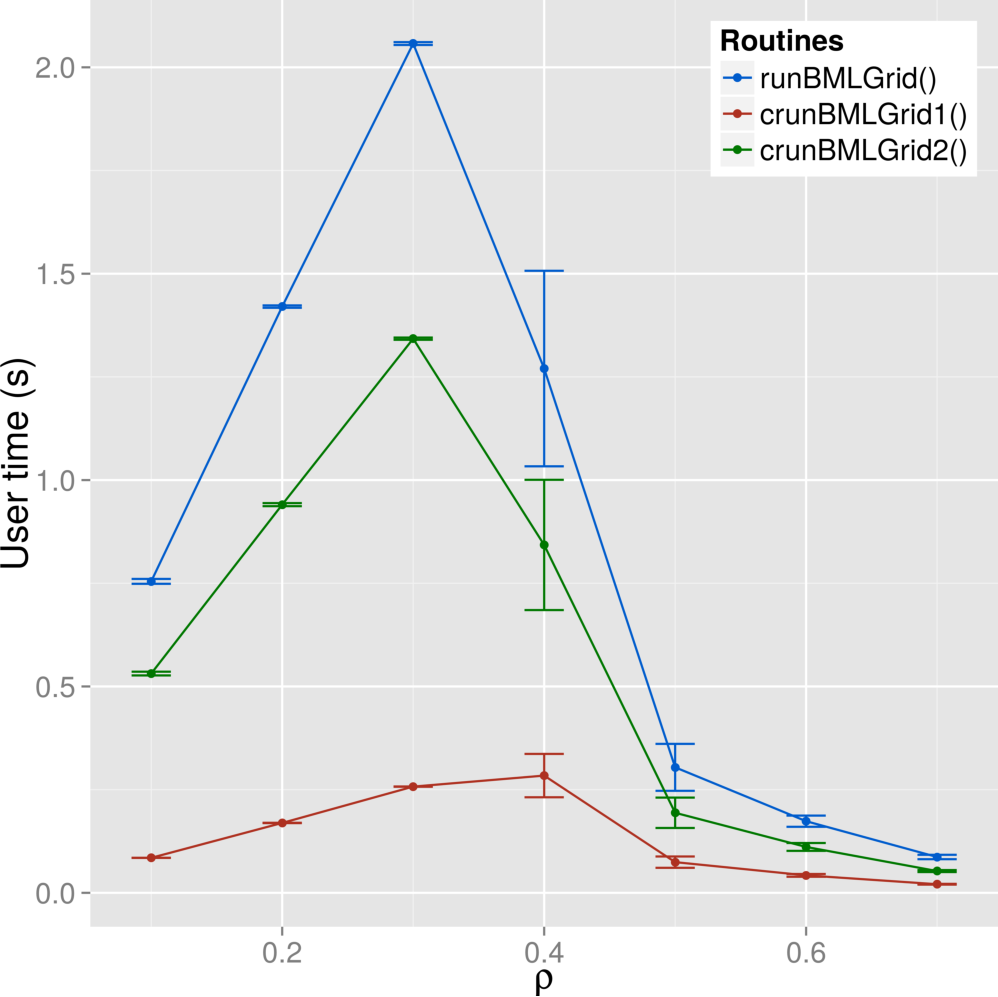
\includegraphics[width=6.0cm]{./figs/TestRunningTime_128.pdf}}
      \centerline{(a) $l = 128$}\medskip
    \end{minipage}
    \hfill
    \begin{minipage}[b]{0.5\linewidth}
      \centering
      \centerline{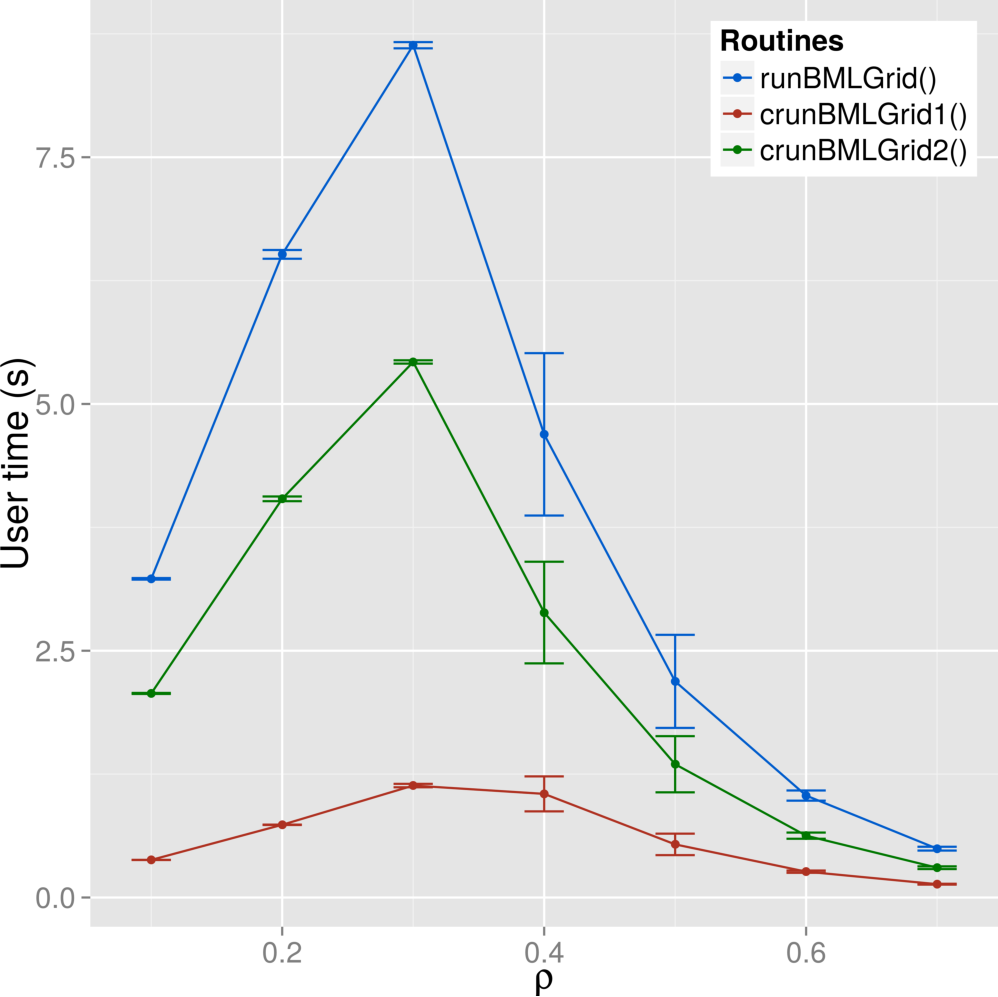
\includegraphics[width=6.0cm]{./figs/TestRunningTime_256.pdf}}
      \centerline{(b) $l = 256$}\medskip
    \end{minipage}
    \hfill
    \begin{minipage}[b]{0.5\linewidth}
      \centering
      \centerline{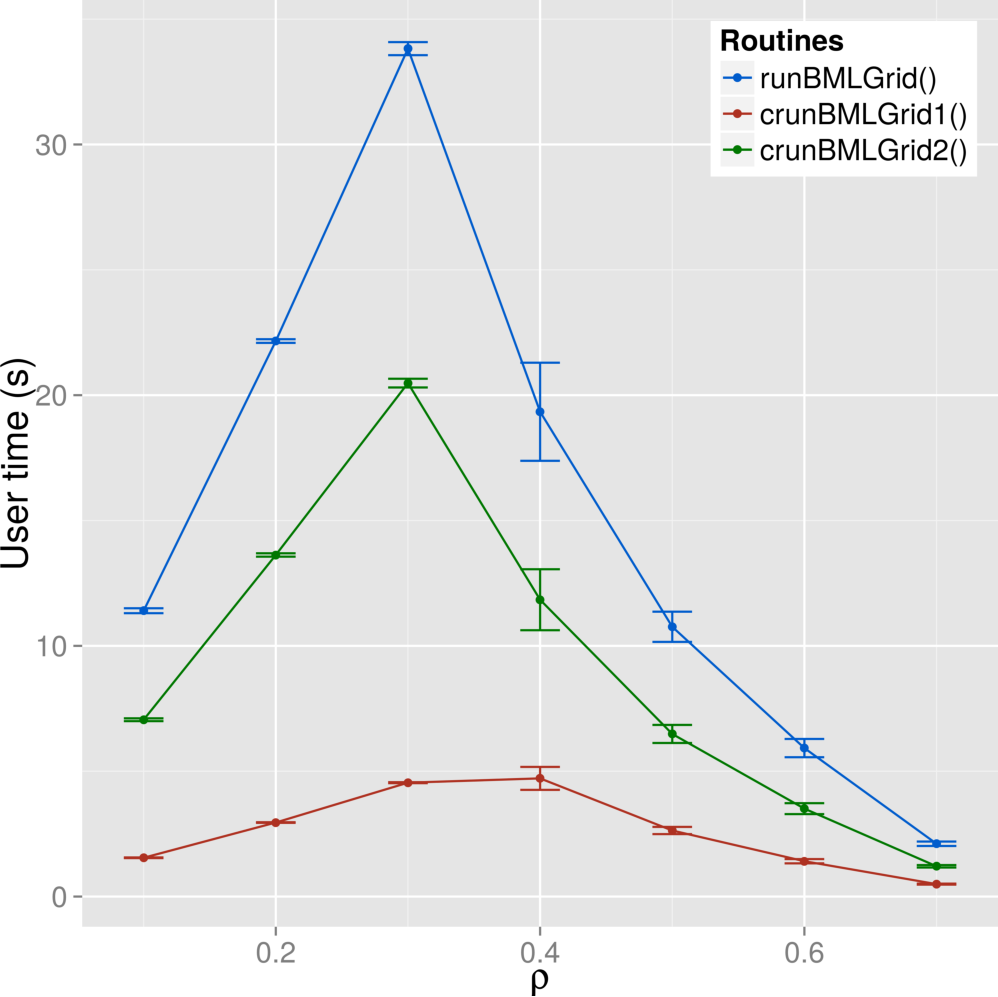
\includegraphics[width=6.0cm]{./figs/TestRunningTime_512.pdf}}
      \centerline{(c) $l=512$}\medskip
    \end{minipage}
    \hfill
    \begin{minipage}[b]{0.5\linewidth}
      \centering
      \centerline{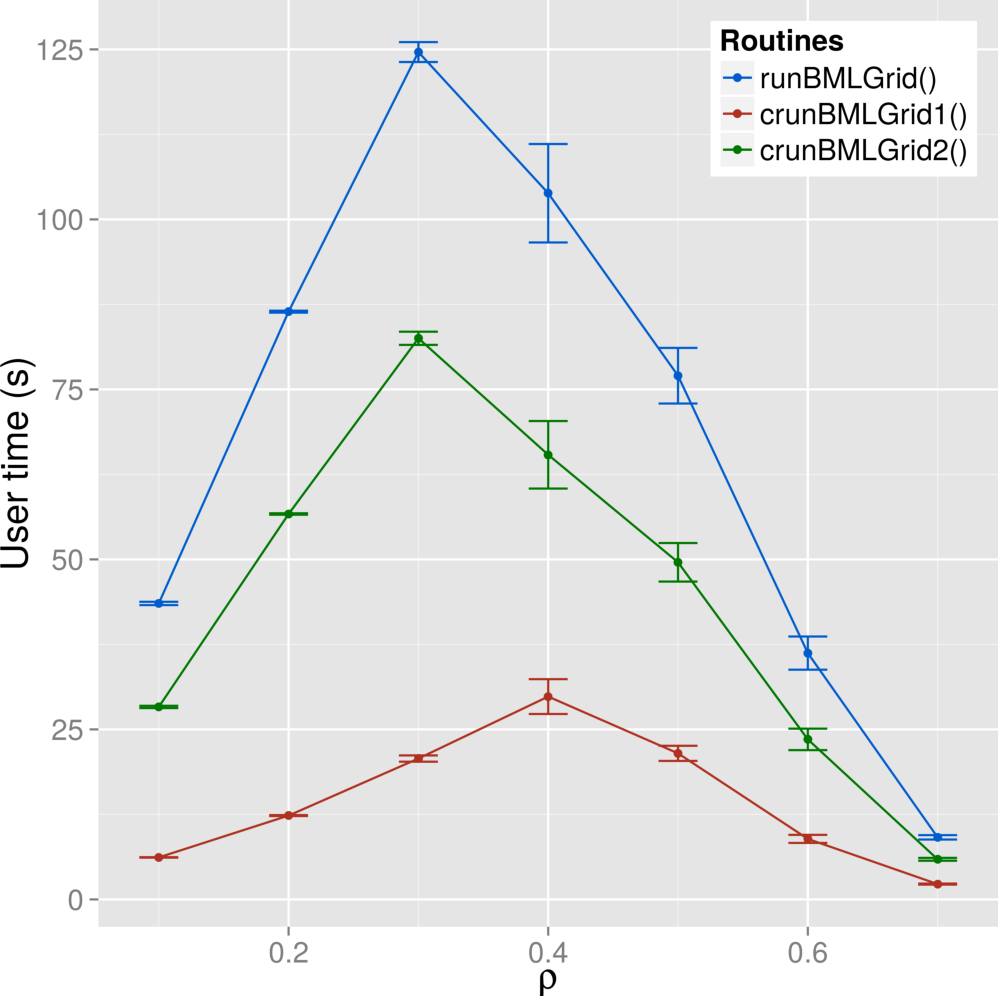
\includegraphics[width=6.0cm]{./figs/TestRunningTime_1024.pdf}}
      \centerline{(d) $l=1024$}\medskip
    \end{minipage}
    \caption{User time comparison between \texttt{runBMLGrid(g, 10000)},
    \texttt{crunBMLGrid1(g, 10000)} and \texttt{crunBMLGrid2(g, 10000)} over 20
    random intial grids for $\rho = 0.1, 0.2, 0.3, 0.4, 0.5, 0.6, 0.7$ and $r =
    c = 128, 256, 512, 1024$.}
    \label{fig:running_time}
\end{figure}

\begin{figure}[H]
    \centering
    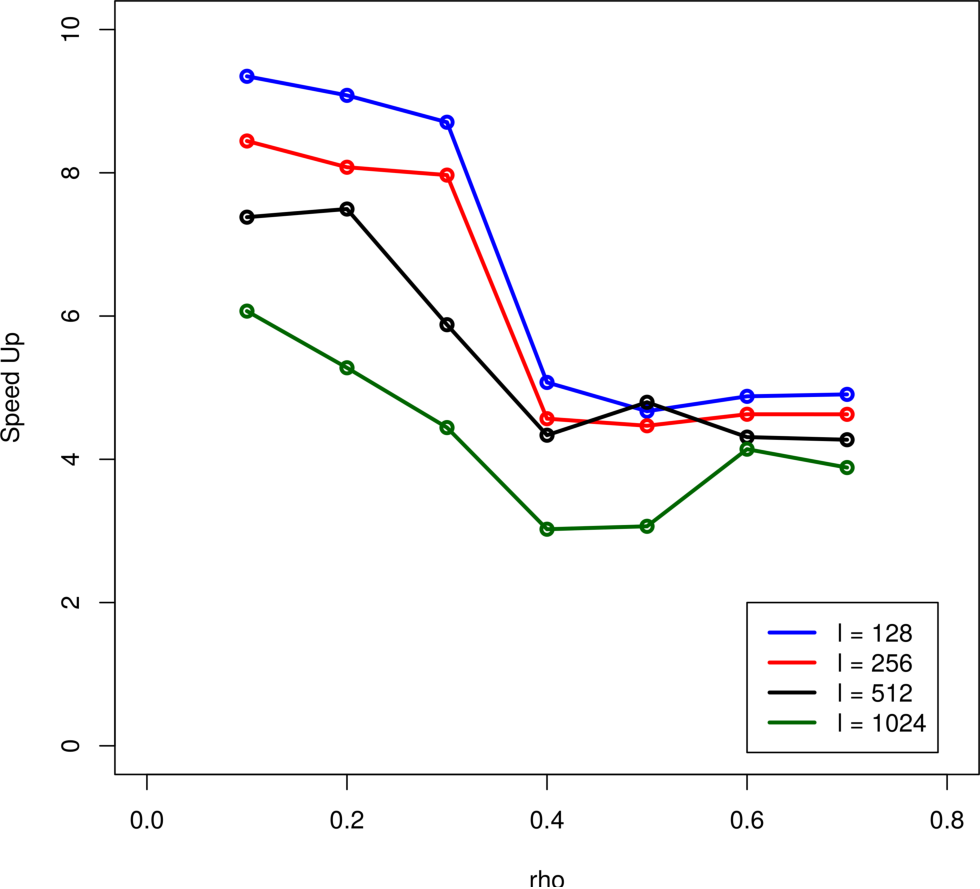
\includegraphics[width=3.5in]{figs/SpeedUp.pdf}
    \caption{Speed up from \texttt{runBMLGrid(g, 10000)} to
    \texttt{crunBMLGrid1(g, 10000)} and \texttt{crunBMLGrid2(g, 10000)} over 20
    random intial grids for $\rho = 0.1, 0.2, 0.3, 0.4, 0.5, 0.6, 0.7$ and $r =
    c = 128, 256, 512, 1024$.}
    \label{fig:speed_up}
\end{figure}

\begin{figure}[H]
    \begin{minipage}[b]{0.5\linewidth}
      \centering
      \centerline{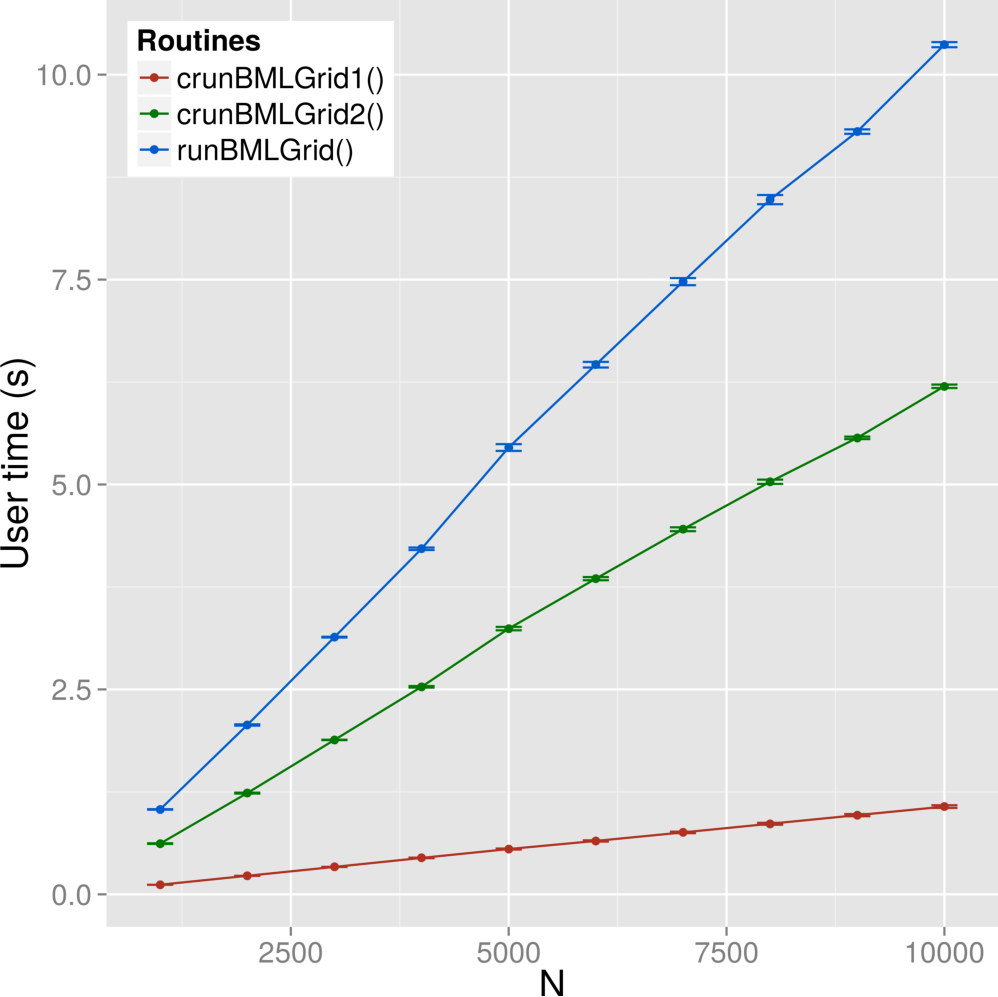
\includegraphics[width=6.0cm]{./figs/TestRunningTimeVsNumStep_03.pdf}}
      \centerline{(a) $\rho = 0.3$}\medskip
    \end{minipage}
    \hfill
    \begin{minipage}[b]{0.5\linewidth}
      \centering
      \centerline{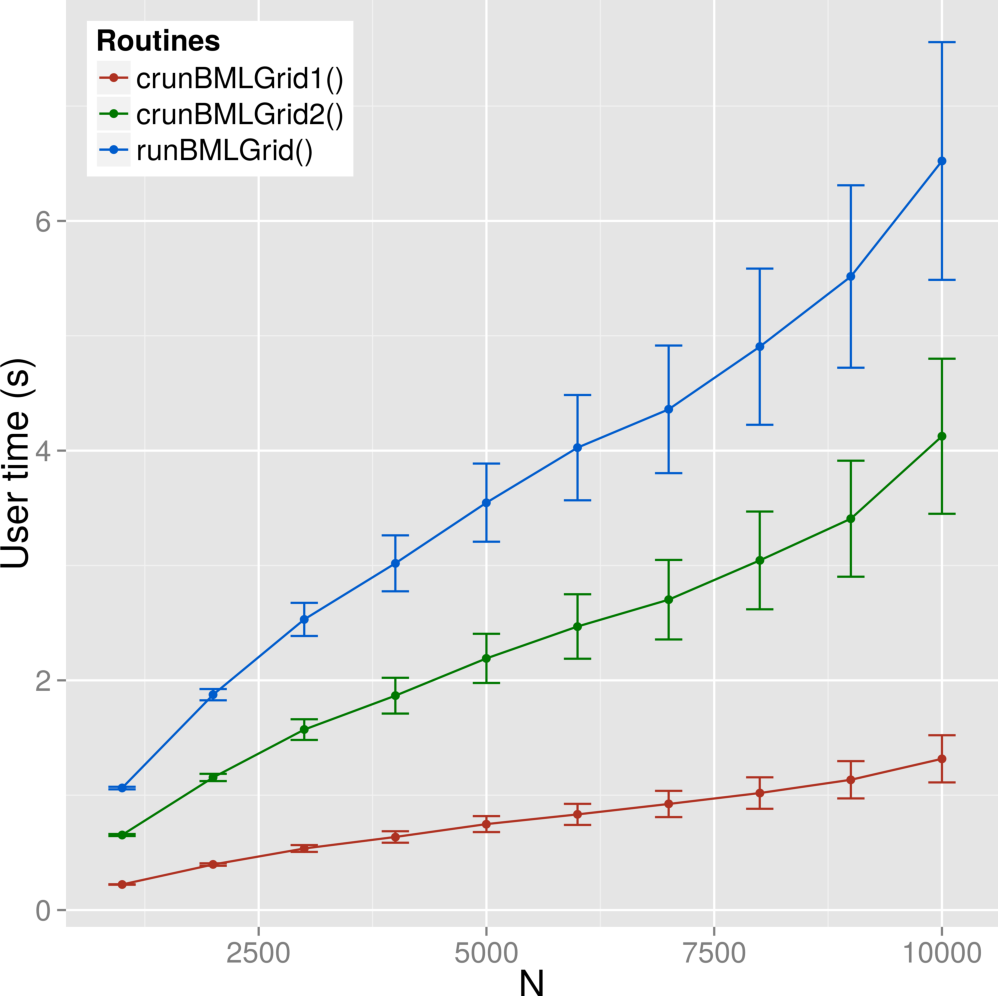
\includegraphics[width=6.0cm]{./figs/TestRunningTimeVsNumStep_04.pdf}}
      \centerline{(b) $\rho = 0.4$}\medskip
    \end{minipage}
    \hfill
    \begin{minipage}[b]{1\linewidth}
      \centering
      \centerline{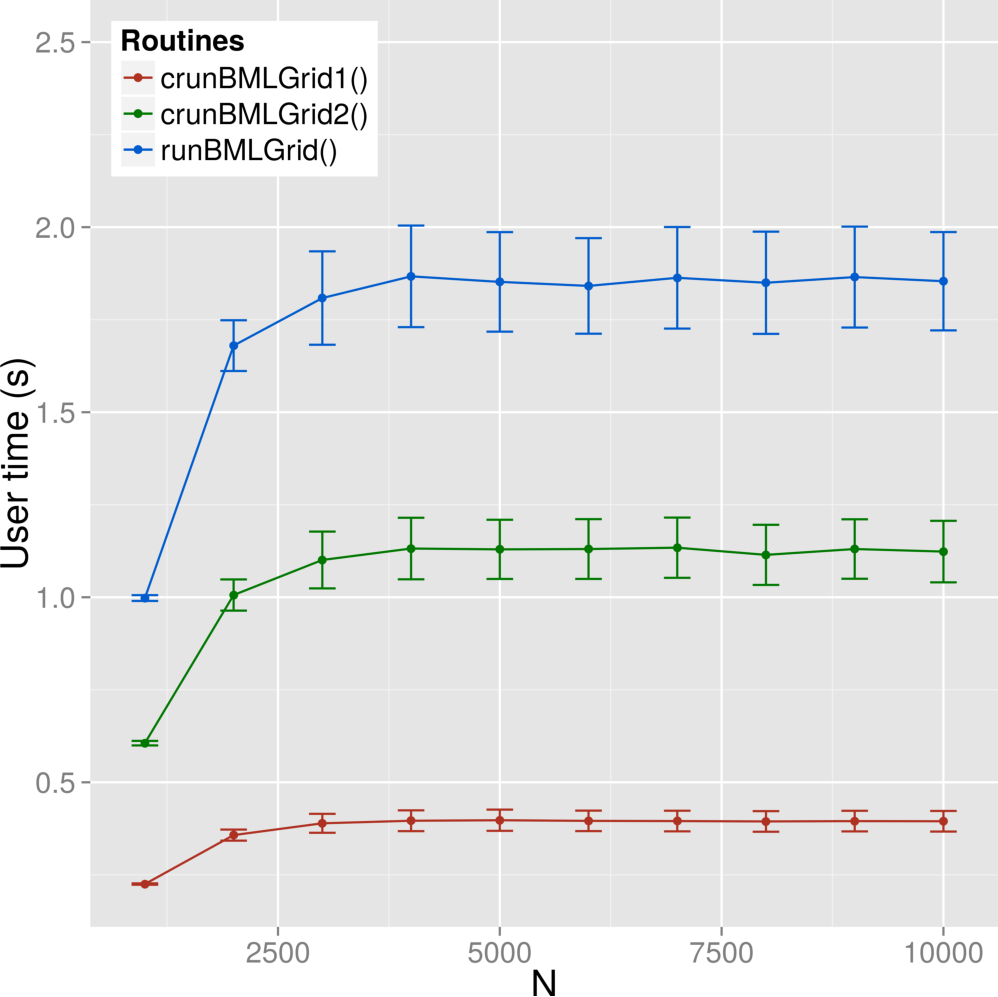
\includegraphics[width=6.0cm]{./figs/TestRunningTimeVsNumStep_05.pdf}}
      \centerline{(c) $\rho = 0.5$}\medskip
    \end{minipage}
    \caption{User time comparison between \texttt{runBMLGrid(g, N)},
    \texttt{crunBMLGrid1(g, N)} and \texttt{crunBMLGrid2(g, N)} over 20
    random intial grids for $\rho = 0.3, 0.4, 0.5$ and $r =
    c = 256$.}
    \label{fig:running_time_vs_numsteps}
\end{figure}
%\pagebreak


\pagebreak
\section*{Appendix: Source Files}
\subsection*{\texttt{BMLGrid.R}}
\lstinputlisting[language=R]{../BMLGrid/R/BMLGrid.R}
\subsection*{\texttt{BMLGrid.h}}
\lstinputlisting[language=C++]{../BMLGrid/src/BMLGrid.h}
\subsection*{\texttt{BMLGrid.cpp}}
\lstinputlisting[language=C++]{../BMLGrid/src/BMLGrid.cpp}


%----------------------------------------------------------------------------------------


\end{document}